\documentclass[11pt]{article}
\usepackage[utf8]{inputenc}
\usepackage{amsfonts}
\usepackage{amsmath}
\usepackage{amsthm}
\usepackage[english]{babel}
\usepackage{booktabs}
\usepackage[labelfont=bf]{caption}
\usepackage{fullpage}
\usepackage{graphicx}
\usepackage[utf8]{inputenc}
\usepackage[numbers]{natbib}
%\usepackage{parskip}
%\usepackage{subcaption}

\usepackage[
  colorlinks=true,
  linkcolor=black,
  anchorcolor=black,
  citecolor=black,
  filecolor=black,
  menucolor=black,
  runcolor=black,
  urlcolor=black]{hyperref}

\title{A Tutorial on Weighted Automata in Machine Learning}
\author{Awni Hannun\footnote{
  Send correspondence to
  \href{mailto:awni.hannun@gmail.com}{awni.hannun@gmail.com}}}

\begin{document}
\maketitle

\begin{abstract}
    Graphs in speech recognition are important.
\end{abstract}

\tableofcontents

\section{Introduction}
\label{sec:introduction}

Relatively speaking, finite-state automata have a long history of application
in machine learning. The majority of these applications involve sequential
data.  For example, they are or have been used in speech recognition, machine
translation and other natural language tasks, and protein function analysis and
other tasks in computational biology.

However, the application of these data structures in machine learning is far
from main stream. In fact, their use likely decreased with the advent of
end-to-end deep learning. The recent development of frameworks for automatic
differentiation with automata suggests there may be renewed interest in the
application of automata to machine learning.

This tutorial introduces weighted automata and their operations. Once this
fundamental data structure is well understood, we then continue to build our
intuition by working through some extended examples.  I hope at minimum this
tutorial engenders an appreciation for the potential of automata in machine
learning. Ideally for some readers this tutorial will be a launching point for
the incorporation of automata in machine-learning research and applications.

However, before launching into the more technical content, let's start with
some broader perspectives in order to motivate the use of automata in machine
learning.

\subsection{Monolithic or Modular}

In the past, complex machine-learning systems, like those used in speech
recognition, involved many specialized hand-engineered components. The trend
is now for the opposite. Most machine-learning applications involve a single,
monolithic neural network. Both of these extremes have advantages and both have
disadvantages.

I believe a primary advantage of automata in machine learning is their
ability to harness the best of both worlds. Automata are capable of retaining
many if not all of the advantages of a multi-component, hand-engineered system
as well as those of a monolithic deep neural network. The next few paragraphs
explain some of these advantages and the regime to which they apply.

\paragraph{Modular:} One of the advantages of multi-component, hand-engineered
systems over monolithic neural networks is modularity. In traditional software
design modularity is usually a good thing. Modular systems are easier to
develop since part of the system can be changed without needing to change the
rest. In machine-learning systems, modularity is useful to avoid retraining the
entire system when only part of the model needs to be updated. Modularity can
also be useful when the individual modules can be reused. For example, speech
recognition systems are built from acoustic models and language models.
Acoustic models can be language agnostic and used for different languages.
Language models are general text based models which can be used in many
different tasks.

\paragraph{Compound errors:} A primary disadvantage of modular systems is that
errors compound. Each module is typically developed in isolation and hence
unaware of the types of errors made by the modules from which it receives
input. Monolithic systems on the other hand can be thought of as being
constructed from many sub-components all of which are jointly optimized towards
a single goal. These sub-components can learn to compensate for the mistakes
made by the others and in general work together more seamlessly.

\paragraph{Adaptable:} Modular systems are typically more adaptable than
monolithic systems. A machine-learning model which is tuned for one domain
usually won't work in another domain without retraining at least part of the
model on data from the new domain. Monolithic neural networks typically require
a lot of data and hence are difficult to adapt to new domains. Modular systems
must also be adapted. However, in some cases only one or a small subset of the
modules need be updated, making the adaptation problem simpler.

\paragraph{Learns from data:} One of the hallmarks of deep neural networks is
their ability to continue to learn and improve with larger data sets. Because
of the many assumptions hard-wired into more traditional modular systems, they
hit a performance ceiling much earlier as data set sizes increase. Retaining
the ability to learn when data is plentiful is a critical features of any
machine-learning system.

\paragraph{Prior knowledge:} On the other hand, one of the downsides of deep
neural networks is their need for large data sets to yield even decent
performance. Encoding prior knowledge into a model improves sample efficiency
and hence reduces the need for data. Encoding prior knowledge into a deep
neural networks is not easy. In some cases, encoding prior knowledge into a
neural network can be done, such as the translation invariance of convolutions.
However, in general, this is not so straightforward. Modular systems by their
very nature incorporate prior knowledge for a give task. Each module is
designed and built to solve a specific sub-task, usually with plenty of
potential for customization towards that task.

Modular and monolithic systems have complementary advantages with respect to
these four traits. Ideally we could construct machine-learning models which
retain the best of each. Automata-based modeling is one possibility which will
task us a step closer towards this goal.  However, to use automata to their
full potential we have to overcome a couple of challenges. The key is enabling
the use of weighted automata in training the model itself. This requires 1)
efficient implementations 2) easy to use frameworks which support automatic
differentiation.

\subsection{Advantages of Differentiable Automata}
\label{sec:advantages}

A key to unlocking the potential of automata in machine learning is enabling
their use during the training stage machine-learning models. All of the
operations I introduce later are differentiable with respect to the arc weights
of their input graphs. This means that weighted automata and the operations on
them can be used in a similar manner as tensors and their corresponding
operations are used in deep learning. Operations can be chained to form complex
computation graphs. Some of the weighted automata which are input to the
computation graph can have parameters which are learned. These parameters can
be optimized using back-propagation and gradient descent.

Automatic differentiation makes computing gradients for complex computation
graphs much simpler. Hence combining automatic differentiation with weighted
automata is important to enabling their use in training machine-learning
models.

Sophisticated machine-learning systems often separate the training and
inference stages of the algorithm. Multiple models are trained in isolation via
one code path. For prediction on new data, the individual models are combined
and rely on a different code path. The constraints of the two regimes (training
and inference) are such that separation from a modeling and software
perspective is often the best option. However, this is not without drawbacks.

First, from a pragmatic standpoint, having separate logic and code paths for
training and inference requires extra effort and usually results in bugs from
subtle mismatches between the two paths. Second, from a modeling standpoint,
optimizing individual models in isolation and then combining them is often
sub-optimal.

One of the benefits of combining automatic differentiation with weighted
automata is the potential to bring the training and inference stages closer
together. For example, speech recognition systems often uses hand-implemented
loss functions at training time. However, the decoder (used for inference)
brings together multiple models represented as graphs (lexicon, language model,
acoustic model, \emph{etc.}) in a completely different code path. By enabling
automatic differentiation with graphs, the decoding stage can also be used for
training.  This has the potential to both simplify and improve the performance
of the system.

Loss functions like Connectionist Temporal Classification, the Automatic
Segmentation criterion, and Lattice-free Maximum Mutual Information are
implemented with custom and highly optimized software. However, these loss
functions can all be implemented using graphs and (differentiable) operations
on graphs.

This separation of code from data, where graphs represent the data and
operations on graphs represent the code, has several benefits. First, the
separation simplifies the software. Second, the separation facilitates research
by making it easier to experiment with new ideas. Lastly, the separation
enables the optimization of graph operations to be more broadly shared.

\subsection{Comparison to Tensors}
\label{sec:comparison_to_tensors}

Modern deep learning is built upon the tensor data structure and the many
operations which take as input one or more tensors. Some of the more common
operations include matrix multiplication, 2-dimensional convolution, reduction
operations, and unary and binary operations.

Automata are an alternative data structure and the operations are quite
different in general. However, one can draw a loose analogy between the
operations on automata and those on tensors.
Table~\ref{tab:tensor_wfst_analogy} shows some of the common operations on
tensors and their analogous operations on automata. The analogy is quite loose,
but still useful at the very least as a mnemonic device and perhaps can help
build intuition for the various operations on graphs.

For example, superficially the formula for matrix multiplication and transducer
composition are quite similar. Assume we have three matrices such that $\mC = \mA
\mB$, then the $(i, j)$ element of $\mC$ is given by:
\begin{equation}
    C_{ij} = \sum_{k} A_{ik} B_{kj}
\end{equation}
Assume we have three transducers (graphs) where $\gC$ is the composition of
$\gA$ and $\gB$ , then the score of the path pair $(\vu, \vv)$ is given by:
\begin{equation}
    \mathcal{C}(\vu, \vv) = \LSE_{\vr} \mathcal{A}(\vu, \vr) + \mathcal{B}(\vr, \vv),
\end{equation}
where $\LSE$ is the \emph{log-sum-exp} operation.
%(we will describe composition
%in much more detail in section~\ref{sec:advanced_operations}).
Both operations take on the form of an accumulation over an inner variable of
values from each of the inputs. In matrix multiplication this is the shared
dimension of the matrices $\mA$ and $\mB$. In graph composition the inner
variable is the shared path $\vr$.

\begin{table}[ht]
    \renewcommand{\arraystretch}{1.4}
    \caption{The table shows loosely analogous operations between tensors and
    automata (acceptors and transducers).}
    \centering
    \begin{tabular}{l l l}
    \toprule
        Tensor & Automata \\
    \midrule
        Matrix multiplication, convolution & Intersect, compose \\
        \rowcolor{Gray} Reduction ops (sum, prod, \emph{etc.}) & Shortest distance (forward, Viterbi) \\
        Unary ops (power, negation, \emph{etc.})  & Unary ops (closure) \\
        \rowcolor{Gray} $n$-ary ops (addition, subtraction, \emph{etc.})  & $n$-ary ops (concatenation, union) \\
    \bottomrule
    \end{tabular}
    \label{tab:tensor_wfst_analogy}
\end{table}

A higher-level analogy to tensor-based deep learning can also be made. Modern
machine-learning frameworks like PyTorch and TensorFlow (and their ancestors
like Torch and Theano) were critical to the success of tensor-based deep
learning. These frameworks include support for automatic differentiation. They
also provide easy to use access to extremely efficient implementations of the
core operations. In the same way, automata-based machine learning should
benefit from frameworks with these features. We are just beginning to see new
developments in frameworks for automata-based machine learning including
GTN\footnote{I am a primary author of the GTN framework which is open source at
\url{https://github.com/gtn-org/gtn}} and K2\footnote{The K2 framework is the
successor of Kaldi and is open source at \url{https://github.com/k2-fsa/k2}}.
Perhaps these will encourage the use of automata in machine learning.

\subsection{History and Bibliographic Notes}

\citet{hopcroft2001introduction} provides an excellent introduction to
non-weighted automata. \citet{mohri2009weighted} gives a more formal and
general treatment of weighted automata and associated algorithms.

Weighted finite-state automata are commonly used in speech recognition, natural
language processing, optical character recognition, and other
applications~\citep{breuel2008ocropus, knight2009applications, mohri1997finite,
mohri2002weighted, mohri2008speech}. \citet{pereira1997} was an early
application of weighted automata to speech recognition, though before that
there were other applications in natural language
processing~\citep{pereira1994weighted, sproat1996stochastic}. The Graph
Transformer Networks of~\citet{bottou97}, a similar though more general
framework, were developed around the same time and applied to character
recognition in images.

The sequence criteria mentioned in section~\ref{sec:advantages}, namely
Connectionist Temporal Classification~\citep{graves2006}, the Automatic
Segmentation criterion~\citep{collobert2016wav2letter}, and Lattice-free
Maximum Mutual Information~\citep{povery2016purely} are most commonly used in
speech recognition. Section~\ref{sec:extended_examples} shows how to implement
a subset of these using weighted automata. \citet{hannun2017sequence} gives a
more detailed introduction to Connectionist Temporal Classification.


In terms of software, two of the better known libraries for operations on WFSTs
are OpenFST~\citep{mohri2000design} and its predecessor
FSM~\citep{allauzen2007openfst}. In section~\ref{sec:comparison_to_tensors} I
compared weighted automata to tensors. PyTorch~\citep{paszke2019pytorch} and
TensorFlow~\citep{abadi2016tensorflow} are two of the most used libraries for
tensor-based deep learning with automatic differentiation. These were based on
earlier frameworks including Torch~\citep{collobert2011torch7} and
Theano~\citep{bergstra2010theano}. Libraries which support automatic
differentiation with weighted automata have only recently been
developed~\citep{k2, hannun2020differentiable}.

\documentclass[main.tex]{subfiles}
\begin{document}

\section{Acceptors and Transducers}
\label{sec:acceptors_transducers}

\subsection{Automata}
\label{sec:automata}

The broad class of graphs we are going to look at are finite-state automata.
These include deterministic finite-state automata (DFAs) and non-deterministic
finite-state automata (NFAs). More specifically we will consider a
generalization of DFAs and NFAs called weighted finite-state acceptors (WFSAs).
That's a mouthful, so I will just call them \emph{acceptors}. We will also consider
a further generalization of an acceptor called a \emph{transducer} (weighted
finite-state transducers or WFSTs). The following figure shows the relation
between these three graphs; transducers, acceptors, and automtata. Transducers
are the most expressive in terms of their representational power, followed by
acceptors followed by unweighted automata.

\begin{figure}
    \centering
    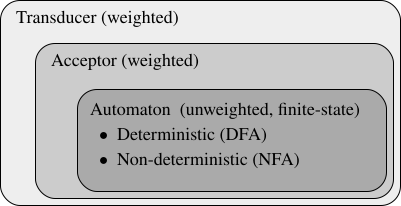
\includegraphics[width=0.5]{wfsa_classes}
    \caption{A hierarchy of automata classes from general to specific in terms
    of representation power. Weighted transducers can represent anything that
    weighted acceptors can represent. Weighted acceptors in turn can represent
    any unweighted finite-state automata.}
    \label{fig:wfsa_classes}
\end{figure}

\end{document}

\section{Basic Operations}
\label{sec:basic_operations}

\section{Advanced Operations}
\label{sec:advanced_operations}


\bibliographystyle{unsrt}
\bibliography{references}

\end{document}
